\documentclass[../Main.tex]{subfiles}

\begin{document}
\author{Progressive Waves} %use author for title of lesson
\date{Year 1 Topic 16} %use date to refer to topic in main booklet

\section{Progressive Waves} %Section is the title of the lesson repeated, ready for the main contents page.

\begin{frame}{Progressive Waves}
    \begin{block}{Definition}
    A wave is an oscillation that travels through matter (or in some cases, a vacuum).  
    \end{block}
    
    \pause
    \begin{block}{Progressive Wave}
    A progressive wave is a wave that has an overall propagation of energy. 
    \end{block}
    
    \pause
    Cast your mind back to GCSE, what examples of waves can you think of?
\end{frame}

\begin{frame}{Transverse Waves}
    What you might picture as a wave is a transverse wave:
    \begin{figure}
        \centering
        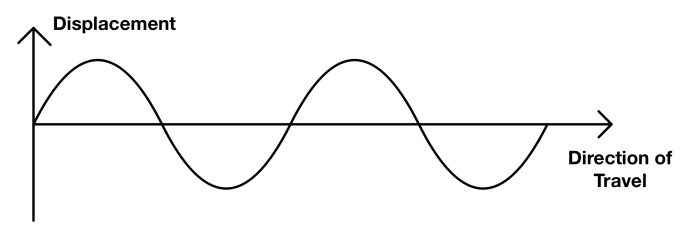
\includegraphics[width=\textwidth]{Waves_Images/transversewave.png}
    \end{figure}
    
    \begin{block}{Transverse Waves}
    In a transverse wave, the direction of oscillation is perpendicular to the direction of motion/energy propagation.
    \end{block}
\end{frame}

\begin{frame}{Longitudinal Waves}
\begin{block}{Longitudinal}
    In a longitudinal wave, the direction of oscillation is parallel to the direction of energy transfer.
    \end{block}
    
    \begin{figure}
        \centering
        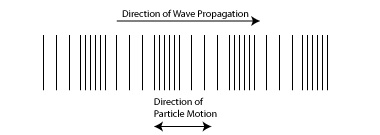
\includegraphics[width=\textwidth]{Waves_Images/longitudinalwave.png}
    \end{figure}
\end{frame}

\begin{frame}{Longitudinal Waves}
    A longitudinal wave can be equated to a transverse wave for the purposes of drawing the wave on paper, with areas of \emph{compression} and \emph{rarefaction} equating to peaks and troughs of a wave. 
    
    \begin{figure}
        \centering
        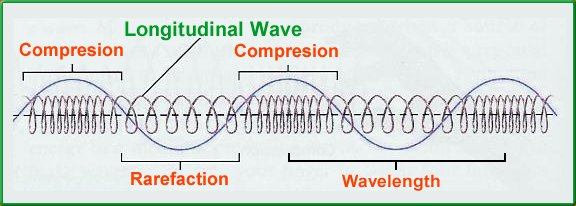
\includegraphics[width=\textwidth]{Waves_Images/rarefaction.png}
    \end{figure}
\end{frame}

\begin{frame}{Properties of waves}
    There are some key definitions for waves that you must know.
    \begin{block}{Wavelength -- $\lambda$}
        The distance between two equivalent points in adjacent wave cycles. Typically found peak to peak, or trough to trough -- units meters
    \end{block}\pause 
    \begin{block}{Amplitude}
    The maximum displacement of a wave -- units meters.
    \end{block}
    \begin{figure}
        \centering
        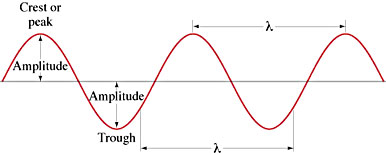
\includegraphics[height=3cm]{Waves_Images/amplitude_wavelength.png}
    \end{figure}
\end{frame}

\begin{frame}{Properties of waves}
    \begin{block}{Frequency}
    The rate at which full cycles of waves pass a single point -- units Hertz (Hz) or $s^{-1}$.
    \end{block}\pause 
    \begin{block}{Time period}
    The time taken for one full wave cycle to pass at a single point -- units seconds.
    \end{block}\pause 
    \begin{block}{Wavespeed}
    The speed of the wave -- units ms$^{-1}$.
    \end{block} \pause 
    --Might these be related at all?
\end{frame}

\begin{frame}{Wave Equation}
    The wavespeed, wavelength, and frequency are all related:
    {\large \begin{equation*}
        v=f\lambda
    \end{equation*}} \pause
    
    In addition, frequency and time period are: 
    
    \begin{equation*}
        f=\frac{1}{T}
    \end{equation*} 
    
    Hence we can also say 
    
    \begin{equation*}
        v=\frac{\lambda}{T}
    \end{equation*}
\end{frame}

\begin{frame}{Examples}
    \begin{exampleblock}{Example 1}
    If a sound wave of frequency 2000Hz is travelling in air, what is its wavelength? \pause
    -- 0.17m
    \end{exampleblock}\pause
    \begin{exampleblock}{Example 2}
    A microwave of frequency 6 GHz is travelling in a vacuum. What is its wavelength? \pause
    --0.05m
    \end{exampleblock}\pause
    \begin{exampleblock}{Example 3}
    Some earthquake waves have the low frequency of 0.2 Hz and a wavelength of 40 km. What is their speed? \pause
    --8kms$^{-1}$.
    \end{exampleblock}
\end{frame}

\end{document}